\documentclass[tikz,border=5pt]{standalone}
\begin{document}
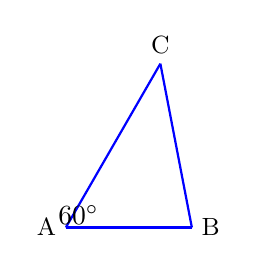
\begin{tikzpicture}[scale=0.8]
    \coordinate (A) at (0,0);
    \coordinate (B) at (2,0);
    \coordinate (C) at (1.5,2.6);

    \draw [blue, thick] (A) -- (B);
    \draw [blue, thick] (A) -- (C);
    \draw [blue, thick] (B) -- (C);

    \node [font=\small, left] at (A) {A};
    \node [font=\small, right] at (B) {B};
    \node [font=\small, above] at (C) {C};

    \node at ([shift={(0.2,0.2)}]A) {$60^\circ$};
\end{tikzpicture}
\end{document}
